\documentclass[tikz]{standalone}
\begin{document}

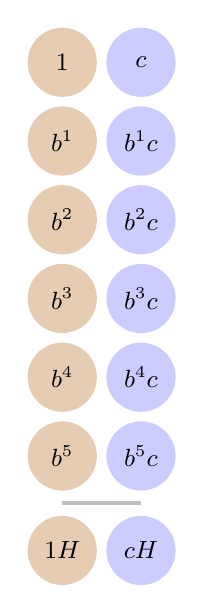
\begin{tikzpicture}
\newcommand{\Radiii}{1}
        \foreach \x in {1,...,5} {
                \node[circle,minimum size=2.5em,fill=blue!20] at (1,{-\Radiii*\x}) {\small\(b^{\x}c\)};
                \node[circle,minimum size=2.5em,fill=brown!40] at (0,{-\Radiii*\x}) {\small\(b^{\x}\)};
		}
        \node[circle,minimum size=2.5em,fill=blue!20] at (1,0) {\small\(c\)};
        \node[circle,minimum size=2.5em,fill=brown!40] at (0,0) {\small\(1\)};        
        \draw [gray!50,ultra thick] (0,{-\Radiii*5.6}) -- (1,{-\Radiii*5.6});
        \node[circle,minimum size=2.5em,fill=blue!20] at (1,{-\Radiii*6.2}) {\small\(cH\)};
        \node[circle,minimum size=2.5em,fill=brown!40] at (0,{-\Radiii*6.2}) {\small\(1H\)};        
        
\end{tikzpicture}
\end{document}
